
\section{等价关系}
\subsection{等价关系}
\begin{definition}
设\(\rel{R}\)是集合\(A\)上的二元关系,即\(\rel{R} \subseteq A^2\).
\begin{itemize}
	\item 对于\(\forall x \in A\),若满足\[
		x\rel{R}x,
	\]
	则称“关系\(\rel{R}\)具有\DefineConcept{自反性}(reflexive)”;

	\item 对于\(\forall x,y \in A\),若\[
		x\rel{R}y \implies y\rel{R}x,
	\]
	则称“关系\(\rel{R}\)具有\DefineConcept{对称性}(symmetric)”;

	\item 对于\(\forall x,y,z \in A\),若\[
		x\rel{R}y \land y\rel{R}z \implies x\rel{R}z,
	\]
	则称“关系\(\rel{R}\)具有\DefineConcept{传递性}(transitive)”.
\end{itemize}
\end{definition}

\begin{example}
%@see: 《Elements of Set Theory》 P61. Exercise 32.
%@see: 《Elements of Set Theory》 P61. Exercise 33.
设\(\rel{R}\)是集合\(A\)上的二元关系.
证明:\begin{enumerate}
	\item \(\rel{R}\)具有对称性的充要条件是\(\rel{R}^{-1} \subseteq \rel{R}\).
	\item \(\rel{R}\)具有传递性的充要条件是\(\rel{R}\circ\rel{R} \subseteq \rel{R}\).
	\item \(\rel{R}\)同时具有对称性和传递性的充要条件是\(\rel{R} = \rel{R}^{-1}\circ\rel{R}\).
\end{enumerate}
%TODO
\end{example}

\begin{definition}
设\(\rel{R}\)是集合\(A\)上的二元关系,即\(\rel{R} \subseteq A^2\).
如果\(\rel{R}\)同时具有自反性、对称性、传递性,
则称“\(\rel{R}\)是\(A\)上的\DefineConcept{等价关系}(equivalence relation)”.
\end{definition}

\subsection{等价类划分}
\begin{theorem}\label{theorem:集合论.划分集合获得等价关系}
%@see: 《Elements of Set Theory》 P56. Theorem 3M
如果关系\(\rel{R}\)具有对称性和传递性,
那么\(\rel{R}\)是\(\fld \rel{R}\)上的等价关系.
\begin{proof}
任意关系\(\rel{R}\)(不论它是三元的还是四元的)都是它的域上的二元关系,
这是因为\[
	\rel{R}
	\subseteq \dom \rel{R} \times \ran \rel{R}
	\subseteq \fld \rel{R} \times \fld \rel{R}.
\]
已知\(\rel{R}\)具有对称性和传递性,
要证\(\rel{R}\)是\(\fld \rel{R}\)上的等价关系,
只需证\(\rel{R}\)在\(\fld \rel{R}\)上具有自反性.
由于\begin{align*}
	x \in \dom \rel{R}
	&\implies
	\exists y \bigl( x \rel{R} y \bigr) \\
	&\implies
	\exists y \bigl( x \rel{R} y \land y \rel{R} x \bigr)
	&(\text{对称性}) \\
	&\implies
	x \rel{R} x,
	&(\text{传递性})
\end{align*}
可知\(\rel{R}\)在\(\dom \rel{R}\)上具有自反性;
同理,\(x \in \ran \rel{R} \implies x \rel{R} x\),
即\(\rel{R}\)在\(\ran \rel{R}\)上具有自反性;
所以,\(\rel{R}\)在\(\dom \rel{R} \cup \ran \rel{R} = \fld \rel{R}\)上具有自反性.
\end{proof}
\end{theorem}
一般而言,如果\(\rel{R}\)是一个在\(A\)上兼具对称性和传递性的关系,
它可能不是在\(A\)上的等价关系.
根据\cref{theorem:集合论.划分集合获得等价关系} 我们知道,
这样的\(\rel{R}\)在\(\fld \rel{R}\)上具有自反性,
但\(\fld \rel{R}\)可能只是\(A\)的一个小小的子集.

利用\cref{theorem:集合论.划分集合获得等价关系},
我们学会通过对集合\(A\)的划分诱导出一个等价关系.
接下来我们来研究怎么逆转这个过程,
也就是说,已知\(A\)上的等价关系,求\(A\)的划分.

\begin{definition}
%@see: 《Elements of Set Theory》 P57. Definition
已知\(\rel{R}\)是一个等价关系.
对于\(x \in \fld \rel{R}\),集合\[
	\Set{ y \given x \rel{R} y }
\]
称为“\(x\)(在关系\(\rel{R}\)下)的\DefineConcept{等价类}%
(the \emph{equivalence class} of \(x\) (\emph{modulo} \(\rel{R}\)))”,
记作\(\rel{R}[x]\)或\([x]_{\rel{R}}\).
把等价类\(\rel{R}[x]\)中的任意一个元素\(y\)称为%
“\(\rel{R}[x]\)的\DefineConcept{代表}(representative)”.

对不强调关系\(\rel{R}\)时,
也可将上述等价类记为\(\overline{x}\)或\([x]\).
\end{definition}

虽然这里把\(\rel{R}[x]\)叫做等价“类”,
实际上它是实实在在的集合,
这一地位可以由子集公理确保无虞,
这是因为\(\rel{R}[x] \subseteq \ran \rel{R}\).

我们还可以进一步构造等价类的集合,例如\[
	\Set{ \rel{R}[x] \given x \in A },
\]
因为这个集合包含于\(\Powerset(\ran \rel{R})\).

根据等价类的定义,容易得到以下性质.
\begin{property}
设\(\rel{R}\)是\(A\)上的一个等价关系,则有:
\begin{enumerate}
	\item \(x \in A
	\implies \rel{R}[x] \neq \emptyset\).

	\item \(x,y \in A
	\implies \rel{R}[x] = \rel{R}[y]
	\lor \rel{R}[x] \cap \rel{R}[y] = \emptyset\).

	\item \(\forall x,y \in A \bigl( \rel{R}[x] = \rel{R}[y]
	\implies x \rel{R} y
	\iff x \in \rel{R}[y] \land y \in \rel{R}[x] \bigr)\).

	\item \(\forall x,y \in A \bigl( \rel{R}[x] \neq \rel{R}[y]
	\implies \rel{R}[x] \cap \rel{R}[y] = \emptyset \bigr)\).
\end{enumerate}
\end{property}


\begin{lemma}\label{theorem:集合论.相等的等价类的代表等价}
%@see: 《Elements of Set Theory》 P57. Theorem 3N
设\(\rel{R}\)是\(A\)上的一个等价关系,\(x,y \in A\),
那么\[
	\rel{R}[x] = \rel{R}[y]
	\iff
	x \rel{R} y.
\]
\begin{proof}
首先,设\(\rel{R}[x] = \rel{R}[y]\).
由于等价关系\(\rel{R}\)具有自反性,\(y \rel{R} y\),\(y \in \rel{R}[y]\);
那么由\(\rel{R}[x] = \rel{R}[y]\)就有\(y \in \rel{R}[x]\);
根据等价类\(\rel{R}[x]\)的定义,便得\(x \rel{R} y\).

然后,设\(x \rel{R} y\).
任取\(t\),若有\(t \in \rel{R}[y]\),
根据等价类\(\rel{R}[y]\)的定义,
必有\(y \rel{R} t\);
再根据假设条件\(x \rel{R} y\),以及等价关系\(\rel{R}\)具有传递性,
立即可得\(x \rel{R} t\);
那么根据等价类\(\rel{R}[x]\)的定义,
就有\(t \in \rel{R}[x]\);
因此,\(\rel{R}[y] \subseteq \rel{R}[x]\).
又因为\(\rel{R}\)具有对称性,
从\(x \rel{R} y\)还可得到\(y \rel{R} x\),
参照上面的推导过程,交换\(x\)和\(y\)符号,
不难得到\(\rel{R}[x] \subseteq \rel{R}[y]\),
所以\(\rel{R}[x] = \rel{R}[y]\).
\end{proof}
\end{lemma}
从\cref{theorem:集合论.相等的等价类的代表等价} 可以看出,
相等等价类的代表等价,代表等价的等价类相等.

\begin{definition}\label{definition:集合论.划分的定义}
%@see: 《Elements of Set Theory》 P57. Definition
设\(A,\Pi\)都是集合.
若\(\Pi\)满足:
\begin{enumerate}
	\item \(\Pi\)中的元素都是\(A\)的非空子集,即\[
		(\forall p \in \Pi)
		[
			p \neq \emptyset
			\land
			p \subseteq A
		].
	\]

	\item \(\Pi\)中的元素两两互斥,即\[
		(\forall p,q \in \Pi)[p \cap q = \emptyset].
	\]

	\item \(A\)中的元素是\(\Pi\)中某个元素的元素,即\[
		(\forall a \in A)
		(\exists p \in \Pi)
		[a \in p]
		\quad\text{或}\quad
		\bigcup\Pi = A.
	\]
\end{enumerate}
则称“\(\Pi\)是\(A\)的一个\DefineConcept{划分}(partition)”.
\end{definition}

\begin{theorem}
%@see: 《Elements of Set Theory》 P57. Theorem 3P
设\(\rel{R}\)是\(A\)上的一个等价关系,那么由所有等价类组成的集合\[
	\Pi = \Set{ \rel{R}[x] \given x \in A }
\]就是\(A\)的一个划分.
\begin{proof}
对于任一等价类\(\rel{R}[x]\),
由于总有\(x \in \rel{R}[x]\),
它永远不可能是空集;
又因为\(\rel{R}\)是\(A\)上的二元关系,\(\rel{R} \subseteq A^2\),
\(\rel{R}[x] \subseteq \ran \rel{R}\),
所以\(\rel{R}[x]\)一定是\(A\)的子集.
因此,\(\Pi\)满足\cref{definition:集合论.划分的定义} 中的第1条和第3条,
也就是说,在这里我们只需要证明第2条:\(\Pi\)中的元素是互不重叠的.
用反证法,设\(\rel{R}[x] \neq \rel{R}[y]\ (x,y \in A)\),
而且存在\(t \in \rel{R}[x] \cap \rel{R}[y]\),
于是有\[
	x \rel{R} t \land y \rel{R} t,
	\quad\text{即}\quad
	x \rel{R} y,
\]
再根据\cref{theorem:集合论.相等的等价类的代表等价},
必有\(\rel{R}[x] = \rel{R}[y]\),
即\(\rel{R}[x],\rel{R}[y]\)是同一个元素,矛盾!
\end{proof}
\end{theorem}

\begin{definition}
%@see: 《Elements of Set Theory》 P58.
设\(\rel{R}\)是\(A\)上的一个等价关系.
集合\[
	\Set{ \rel{R}[x] \given x \in A }
\]称为“\(A\)在\(\rel{R}\)下的\DefineConcept{划分}”,
或称为“\(A\)对\(\rel{R}\)的\DefineConcept{商集}(quotient set)”,
记作\(A/\rel{R}\),读作“\(A\)余\(\rel{R}\)(\(A\) modulo \(\rel{R}\))”.
把映射\[
	\varphi\colon A \to A/\rel{R}, x \mapsto \rel{R}[x]
\]称为\DefineConcept{自然映射}(natural map)%
或\DefineConcept{典范映射}(canonical map).
\end{definition}
对于一个非空集合\(A\),通过建立\(A\)上的一个等价关系\(\rel{R}\),
得到\(A\)对于\(\rel{R}\)的商集\(A/\rel{R}\),
进而研究商集\(A/\rel{R}\)的性质,
这就是抽象代数的基本方法之一.

现在我们来研究如何在商集上定义映射.
具体而言,设\(\rel{R}\)是\(A\)上的一个等价关系,
映射\(F\colon A \to A\).
我们想知道是否存在一个对应的映射\(\hat{F}\colon A/\rel{R} \to A/\rel{R}\),
使得对于任意\(x \in A\),总有\[
	\hat{F}(\rel{R}[x]) = \rel{R}[F(x)].
\]
这里我们可以尝试依靠在等价类\(\rel{R}[x]\)中选择某个特定的元素\(x\),
定义等价类\(\rel{R}[x]\)在映射\(\hat{F}\)下的值.
不过,假如\(x_1,x_2\)都在同一个等价类中,
那么除非\(F(x_1),F(x_2)\)也都在同一个等价类中,
否则映射\(\hat{F}\)就不是良定的!

为了给出一个一般性结论,我们先了解这样一个概念:
如果\[
	\forall x,y \in A \bigl(
		x \rel{R} y
		\implies
		\opair{F(x),F(y)} \in \rel{R}
	\bigr),
\]
那么我们称“\(F\)和\(\rel{R}\) \DefineConcept{兼容}%
(\(F\) is \emph{compatible} with \(\rel{R}\))”.

\begin{theorem}\label{theorem:集合论.与等价关系兼容的映射的性质}
%@see: 《Elements of Set Theory》 P60. Theorem 3Q
设\(\rel{R}\)是\(A\)上的一个等价关系,映射\(F\colon A \to A\).
如果\(F\)和\(\rel{R}\)兼容,
那么存在一个唯一的映射\(\hat{F}\colon A/\rel{R} \to A/\rel{R}\),使得\[
	\forall x \in A:
	\hat{F}(\rel{R}[x]) = \rel{R}[F(x)].
\]
如果\(F\)和\(\rel{R}\)不兼容,
那么不存在映射\(\hat{F}\)满足上述条件.
\begin{proof}
首先假设\(F\)和\(\rel{R}\)不兼容,即\[
	\exists x,y \in A \bigl(
		x \rel{R} y,
		\opair{F(x),F(y)} \notin \rel{R}
	\bigr),
\]
也即\[
	\exists x,y \in A \bigl(
		\rel{R}[x] = \rel{R}[y],
		\rel{R}[F(x)] \neq \rel{R}[F(y)]
	\bigr).
\]
而要使\[
	\forall x \in A:
	\hat{F}(\rel{R}[x]) = \rel{R}[F(x)]
\]成立,必须有\[
	\hat{F}(\rel{R}[x])
	= \rel{R}[F(x)]
	\quad\text{和}\quad
	\hat{F}(\rel{R}[y])
	= \rel{R}[F(y)]
\]同时成立,
但这是不可能的,
毕竟上面两式的左边相等而右边不等.

接下来,我们假设\(F\)和\(\rel{R}\)兼容.
由于结论要求\(\opair{\rel{R}[x],\rel{R}[F(x)]} \in \hat{F}\),
所以我们可以令\[
	\hat{F} = \Set{ \opair{\rel{R}[x],\rel{R}[F(x)]} \given x \in A }.
\]
现在就需要证明关系\(\hat{F}\)是一个映射.
考虑\(\opair{\rel{R}[x],\rel{R}[F(x)]},
\opair{\rel{R}[y],\rel{R}[F(y)]} \in \hat{F}\),
由于\begin{align*}
	\rel{R}[x] = \rel{R}[y]
	&\implies
	x \rel{R} y
	&(\text{\cref{theorem:集合论.相等的等价类的代表等价}}) \\
	&\implies
	\opair{F(x),F(y)} \in \rel{R} \\
	&\implies
	\rel{R}[F(x)] = \rel{R}[F(y)],
	&(\text{\cref{theorem:集合论.相等的等价类的代表等价}})
\end{align*}
\(\hat{F}\)是单值的,
可见\(\hat{F}\)确实是一个映射.
显然有\(\dom \hat{F} = A/\rel{R}\),\(\ran \hat{F} \subseteq A/\rel{R}\),
因此\(\hat{F}\)是从\(A/\rel{R}\)到\(A/\rel{R}\)的映射.
%TODO 没有给出唯一性的证明
\end{proof}
\end{theorem}
上述结论还可以推广到映射是\(F\colon A \times A \to A\)的情形.



\section{排序关系}
不同于等价关系,\DefineConcept{排序关系}(ordering relation)具有一些别致的性质.

\subsection{线性序}
\begin{definition}
设\(A\)是集合,\(\rel{R}\)是\(A\)上的一个二元关系.
如果\begin{enumerate}
	\item \(\rel{R}\)具有传递性,
	\item \(\rel{R}\)在\(A\)上服从\DefineConcept{三一律}(trichotomy),
	也就是说,对于\(\forall x,y \in A\),
	在以下三个命题中,有且仅有一个是真命题:\[
		x \rel{R} y, \qquad
		x = y, \qquad
		y \rel{R} x;
	\]
	%@see: https://mathworld.wolfram.com/TrichotomyLaw.html
\end{enumerate}
那么称\(\rel{R}\)为%
“\(A\)上的\DefineConcept{线性序}(linear ordering)%
或\DefineConcept{全序}(total ordering)”.
\end{definition}

应该注意到,当\(x = y\)时,三一律要求\[
	x \rel{R} x, \qquad
	x = x, \qquad
	x \rel{R} x
\]中的一个成立,
考虑到\(x = x\)恒成立,
那么必有\(x \rel{R} x\)恒不成立.
易见当\(x \neq y\)时,必有\(x \rel{R} y\)或\(y \rel{R} x\)之一成立,
都不可能有\(x \rel{R} y\)和\(y \rel{R} x\)都成立.
于是我们证得如下定理.

\begin{theorem}
%@see: 《Elements of Set Theory》 P63. Theorem 3R
设\(\rel{R}\)是集合\(A\)上的线性序.
\begin{enumerate}
	\item {\rm \(\rel{R}\)具有\DefineConcept{反自反性}(irreflexive)},
	即不存在\(x\)使得\(x \rel{R} x\).

	\item {\rm \(\rel{R}\)在\(A\)上是连通的(\(\rel{R}\) is \emph{connected} on \(A\))},
	即对于不同的\(x,y \in A\),要么有\(x \rel{R} y\)成立,要么有\(y \rel{R} x\)成立.
\end{enumerate}
\end{theorem}

值得注意的是,
线性序\(\rel{R}\)永远不会给出如下的环形:
\begin{center}
	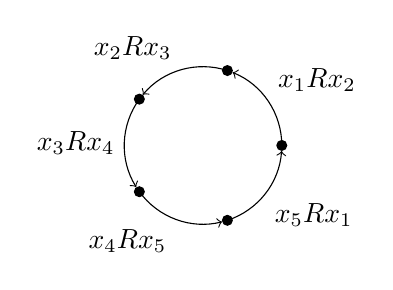
\begin{tikzpicture}
		\fill(1,0)circle(2pt)coordinate(A0);
		\fill({cos(72)},{sin(72)})circle(2pt)coordinate(A1);
		\fill({cos(144)},{sin(144)})circle(2pt)coordinate(A2);
		\fill({cos(216)},{sin(216)})circle(2pt)coordinate(A3);
		\fill({cos(288)},{sin(288)})circle(2pt)coordinate(A4);
		\begin{scope}[->]
			\draw(A0)arc[start angle=0,end angle=68,radius=1]node[midway,above right]{\(x_1 \rel{R} x_2\)};
			\draw(A1)arc[start angle=72,end angle=140,radius=1]node[midway,above left]{\(x_2 \rel{R} x_3\)};
			\draw(A2)arc[start angle=144,end angle=212,radius=1]node[midway,left]{\(x_3 \rel{R} x_4\)};
			\draw(A3)arc[start angle=216,end angle=284,radius=1]node[midway,below left]{\(x_4 \rel{R} x_5\)};
			\draw(A4)arc[start angle=288,end angle=356,radius=1]node[midway,below right]{\(x_5 \rel{R} x_1\)};
		\end{scope}
	\end{tikzpicture}
\end{center}
这是因为,如果我们有这样的环形成立,
那么根据传递性必有\(x_1 \rel{R} x_1\),
而这就与反自反性矛盾!

\begin{example}
设\(\rel{R}\)是\(A\)上的一个线性序,
证明:\(\rel{R}^{-1}\)也是\(A\)上的线性序.
\begin{proof}
由于\[
	\bigl( x \rel{R} y \land y \rel{R} z \implies x \rel{R} z \bigr)
	\iff
	\bigl( y \rel{R}^{-1} x \land z \rel{R}^{-1} y \implies z \rel{R}^{-1} x \bigr),
\]
可知\(\rel{R}^{-1}\)具有传递性.
又因为\(\rel{R}\)是\(A\)上的线性序,
所以对于\(\forall x,y \in A\),以下三个命题\[
	x \rel{R} y, \qquad
	x = y, \qquad
	y \rel{R} x
\]有且仅有一个成立;
换句话说,以下三个命题\[
	y \rel{R}^{-1} x, \qquad
	x = y, \qquad
	x \rel{R}^{-1} y
\]有且仅有一个成立;
可知\(\rel{R}^{-1}\)服从三一律.
综上所述,\(\rel{R}^{-1}\)也是\(A\)上的线性序.
\end{proof}
\end{example}

\subsection{偏序关系}
\begin{definition}
设\(\rel{R}\)是集合\(A\)上的二元关系,即\(\rel{R} \subseteq A^2\).
对于\(\forall x,y \in A\),若\[
	x\rel{R}y \land y\rel{R}x \implies x = y,
\]
则称“关系\(\rel{R}\)具有\DefineConcept{反对称性}(antisymmetric)”.
\end{definition}

\begin{definition}
设\(\rel{R}\)是集合\(A\)上的二元关系,即\(\rel{R} \subseteq A^2\).
如果\(\rel{R}\)同时具有自反性、反对称性、传递性,
则称“\(\rel{R}\)是\(A\)上的\DefineConcept{偏序关系}(ordering relation)”.
\end{definition}

